\documentclass[titlepage]{article}
\usepackage[pdftex]{graphicx}

% Title
\title{Lab 2: Waves}
\author{Yacin Nadji}
\date{October 1st, 2006}

\begin{document}
\maketitle

\section{Statement of Objective}\label{sec:obj}
The purpose of this lab was to view the properties of standing waves generated by an electric field and interfering waves using sound waves. The relationships between the two will also be looked at in order to get a better idea of waves in general. The relationships and properties will be justified using data collected in the lab.

\section{Theory}\label{sec:theory}
Waves exist all around us, so naturally, they are a common object of study. In this lab, we are looking at a specific type of wave called ``standing waves''. Standing waves consist of waves that oscillate about fixed points, called nodes, that never move, and anti-nodes, the area located halfway between each node. This is represented by the variable $n$ and denotes the harmonic of the wave. By determining the harmonic and frequency of any standing wave, one can calculate the velocity, $v$, of the standing wave using this equation:

\begin{equation}
	v = \frac{2 L f}{n}
\end{equation}

Based on this, you could represent the slope of $f$ versus $n$ as:

\begin{equation}
	slope = \frac{v}{2L} = \frac{f}{n}
\end{equation}

Interfering waves occur everywhere in two major forms, constructive waves while in phase, and destructive waves while out of phase. If the difference between the distances the two waves travel to the same point $(S_1b)$ is:

\begin{equation}
	S_1b = m \lambda
\end{equation}

then the waves are constructive, but if the difference is:

\begin{equation}
	S_1b = (m + \frac{1}{2}) \lambda
\end{equation}

then the waves will be destructive. By plotting the $sin(\theta)$ vs. $m$, the wavelength of these waves can be found using:

\begin{equation}
	slope = \frac{\lambda}{d} = \frac{sin \theta}{m}
\end{equation}

Where $d$ is the distance between the waves and the point $P$ when it is centered between the wave's points of origin.

\section{Equipment List}\label{sec:equipment_list}
\begin{itemize}
\item[*] Power Supply
\item[*] Transistor
\item[*] Magnet
\item[*] Hanging Mass
\item[*] Amp Meter
\item[*] Sine Generator
\item[*] Wire String
\item[*] Pulley Setup
\item[*] Anchor Post
\item[*] Measuring Stick
\item[*] Two Speakers
\item[*] Microphone
\item[*] Two Anchor Tracks
\item[*] Oscilloscope
\item[*] Frequency Generator
\end{itemize}

\section{Procedure}\label{sec:procedure}
Refer to Physics 221 Lab Manual for Lab \#2 for the procedure.

\section{Data}\label{sec:data}
\subsection{Part A}\label{sub:part_a}

Frequencies for waves with $n$ nodes:\\
\\
\begin{tabular}{cccc}
\hline
n & f (theoretical) & f (experimental) & \% difference\\
\hline
3 & 60.8 Hz & 60.0 Hz & 1.3 \%\\
\hline
4 & 81.1 Hz & 83.1 Hz & 2.4 \%\\
\hline
5 & 101.4 Hz & 101.4 Hz & 0.0 \%\\
\hline
6 & 141.9 Hz & 142.5 Hz & 0.4 \%\\
\hline
\end{tabular}

\subsection{Part B}\label{sub:part_b}

Distance from center where waves interfere with each other:\\
\\
\begin{tabular}{ccccc}
\hline
M & X_g & X_R & (X_R + X_1)/2 & \theta\\
\hline
1 & 5.4 cm & 8 cm & 6.7 cm & 6.9^o\\
\hline
2 & 11.7 cm & 14.1 cm & 12.9 cm & 13.1^o\\
\hline
3 & 18.5 cm & 21.6 cm & 20.05 cm & 19.9^o\\
\hline
\end{tabular}

\section{Analysis of Data}\label{sec:analysis_of_data}
\\
\\
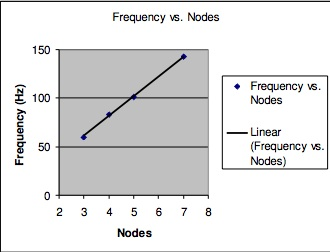
\includegraphics{partA.jpg}
\\
\\
The theoretical speed of the wave should be $36.1 \frac{m}{s}$. The speed we found doing the experiment using $\frac{f}{n} = 20.47$ is $36.34 \frac{m}{s}$.

\[
	\% Error = \frac{|36.34 - 36.1|}{36.1} * 100 = 0.66\%
\]

\\
\\
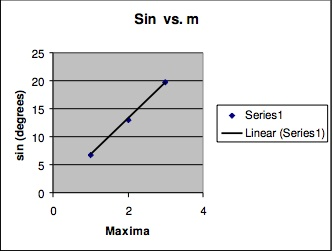
\includegraphics{partB.jpg}
\\
\\
We assumed room temperature to be equal to $296.5 K$ and by using the equation $v = 20.05(T)^{\frac{1}{2}} = 345.24 \frac{m}{s}$. Therefore, $\lambda_{actual} = .0084 m$, where our experimental value is $\lambda_{exp} = .00825$.

\[
	\% Error = \frac{|338.25 - 345.24|}{345.24} * 100 = 2.02\%
\]
\[
	\% Error = \frac{|.00825 - .0084|}{.0084} * 100 = 1.79\%
\]

\section{Discussion of Results}\label{sec:discussion_of_results}
\subsection{Part A}\label{sub:part_a}
Throughout our experimentation we found a wave with velocity: $v = 36.34 \frac{m}{s}$ with a very nice percent error of 0.66 \%. Naturally, due to human error, it's pretty understandable that we were 100 \% accurate, however, an error this small is definitely very good.

\subsection{Part B}\label{sub:part_b}
Part B, not to be outdone by Part A, also yielded wonderful results. We calculated the wave's velocity to be: $v = 338.25 \frac{m}{s}$ and a wavelength of: $\lambda = .00825 m$. These values gave us the percent error of 2.02 \% and 1.79 \%, respectively. Much like Part A, with nice, small percent error values like this, it's apparent the experiments are a good way to reinforce the theories we've learned in class. Due to error on our part, it's easy to see why there's a slight discrepancy between the calculated values, and the experimental values.

\section{Conclusions}\label{sec:conclusions}
The relatively accurate and consistent results provided by our data reinforces the validity of the equations presented to us in class. You can see this by looking at the tables for Part A and B. It is very clear that the linear regression is quite accurate based on our data. In addition to this, our very small percent errors show the numbers we were getting aren't just pulled out of nowhere. It's an understatement to call this lab merely a success.

\end{document}